\section{Background}
\label{sec:background}
Despite recent interest, concerns about system power have existed since the dawn of computing. Some of the earliest valve-based computers had power draws comparable to modern supercomputers. The ENIAC machine dissipated 174 kW \cite{birnbaum:2000aa}, a figure which would not look out of place in the current Top 500 list, despite the fact this machine dates from 1947.\golden

Bipolar semiconductor technologies superseded thermionic valves in the 1950s and 60s, leading to dramatic reduction in power consumption. Over time, manufacturing improvements delivered ever smaller transistors, yielding rapid increases in both performance and power density. Ultimately this resulted in chips which strained the limits of cooling technologies~\cite{jouppi:1994aa}. \golden

The use of bipolar semiconductors peaked in the early 1990s when they were replaced in turn with the Complementary Metal Oxide Semiconductor (CMOS) technology we still rely on today. CMOS was already mature before this point, however it had been viewed as too slow to be of use in high-performance microprocessors. \golden

\begin{figure}[ht]
\centering
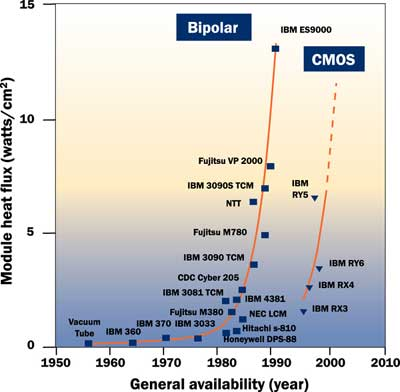
\includegraphics[width=0.9\linewidth]{Images/bipolarcmos.jpg}
\caption{Trends in module level power density, reproduced from \cite{chu:1999aa}. Copyright 1999 IEEE.}
\end{figure}
This pattern of improving hardware until physical limits forces a switch to novel technologies is a recurring one. The previous iteration saw the widespread adoption of multi-core architectures, and once again we find ourselves struggling with the limitations of current hardware \cite{esmaeilzadeh:2011aa}. Unfortunately this time we lack a mature semiconductor technology or architectural paradigm waiting in the wings. Researchers are therefore searching for alternative ways to combat the rise of power consumption and ensure continued benefit from technology scaling whilst we await the emergence of the next fundamental shift in processor technology. \golden

System architects are already focussing on power efficient chip design, with recent innovations in areas including on-die voltage regulation \cite{burton:2014aa}, Dynamic Voltage and Frequency Scaling (DVFS) scheduling \cite{kwon:2013aa} and energy efficient heterogeneous cores~\cite{gupta:2012aa} amongst others. Performance engineers working with standard hardware are also beginning take note of this issue as it becomes increasingly central to scientific computing. It is their efforts to improve software power consumption that we hope to guide in this paper, and so we now limit our discussion to considering commodity CMOS chips with conventional architectures.

The power draw of CMOS chips can be split into distinct components, the most significant of which are dynamic power and leakage power. Dynamic power can be thought of as the power consumed as logic gates change state when a processor performs work. Leakage power dissipation stems from the fact that at very small scales the insulating properties of silicon break down, allowing some current to flow even when gates remain inactive. Other forms of power dissipation do exist, however they are relatively insignificant in terms of magnitude. 




\begin{equation}
\label{eq:totpwr}
P_{tot} = P_{dyn} + P_{leak} + P_{other}
\end{equation}
\begin{equation} 
\label{eq:dynpwr}
P_{dyn} \propto CV^{2}Af
\end{equation}
\begin{equation}
\label{eq:leakpwr}
P_{leak} \propto V\left(ke^{\frac{-qV_{th}}{ak_{a}T}}\right)
\end{equation}

Equations~\ref{eq:dynpwr} and \ref{eq:leakpwr} give relations for dynamic and sub-threshold leakage power respectively. In Equation~\ref{eq:dynpwr}, C denotes load capacitance (a property influenced by wire lengths of on-chip structures), $V$ the supply voltage, $A$ the activity factor and $f$ the clock frequency. There is also a link between $V$ and $f$, as higher clock frequencies require higher supply voltages.

Equation~\ref{eq:leakpwr} is a simplified equation for sub-threshold leakage power. The new terms introduced in this equation include $T$, temperature, $V_{th}$, the transistor threshold voltage and $k$ the Boltzmann constant. The remaining parameters $q$, $a$ and $k_{a}$ capture CMOS logic design and fabrication characteristics. There several other sources of leakage energy, however we omit them for reasons which will  become clear shortly.

Dynamic power draw was historically the biggest contributor to $P_{tot}$, however since the breakdown of Dennard scaling leakage power has been on track to overtake it.  Sub-threshold and gate-oxide leakage dominate total leakage current, with both increasing exponentially as transistors shrink. Process improvements like the introduction of high-k dielectric materials~\cite{jan:2009aa} have kept leakage power in check over the last decade, however there is no avoiding the fact that insulating properties degrade as transistors get smaller, allowing more current to leak.

An important feature of the equations governing power draw is that only $P_{dyn}$ directly depends on the properties of the software running via the $A$ term. Software can indirectly effect leakage current if it blocks frequently, triggering a reduction in clock frequency and therefore a knock on effect on supply voltage. This effect is however primarily one of clock frequency rather than software and will be modelled as such. This is especially true for scientific codes which do not typically leave the processor sitting idle for significant periods.

The final thing to consider before progressing to software optimization is the metric which is to be optimized. Code optimisation is a complex task during which developers typically rely on the support of a range tools and techniques including profilers and performance models. Up until now the overarching goal of performance engineers has been to minimize a single metric - run time. New metrics must be incorporated into these tools in order to support multi-objective optimization encompassing both power and runtime.

Energy to completion is an obvious choice for domains where energy is severely restricted, for example in mobile platforms. It can also be used to understand the amount of heat a chip generates which can be of use to system architects. The fact that this metric fails to consider runtime however reduces its utility in scientific computing domains.

In practice the metrics often selected in this field are variants of the energy-delay product (EDP) \cite{gonzales:1995aa}. If either the runtime or energy consumption of a code increase then its EDP will increase proportionately as both components equally weighted. EDP can be defined in various equivalent ways:

\begin{equation}
EDP = Energy \times Runtime
\end{equation}
\begin{equation}
EDP = Power \times Runtime^{2}
\end{equation}
\begin{equation}
EDP = Power \times (Instructions / MIPS)^{2}
\end{equation}


Following on from the original proposal, related methods such including energy-delay-squared product ($ED^{2}P$) and energy-delay-cubed product ($ED^{3}P$). It can be argued that $ED^{2}P$ is a good choice when considering a fixed micro-architecture \cite{brooks:2000aa}. From equations \ref{eq:totpwr} and \ref{eq:dynpwr} we know that $P_{tot} \propto CV^{2}Af + P_{leak} $, which for a fixed system and workload simplifies to $P_{tot} \propto V^{3}$. We also know that performance and clock frequency are related, meaning performance is roughly proportional to voltage. As a result we have $\frac{runtime^{3}}{P_{tot}} \approx 1$. This demonstrates that $Power \times Runtime^{3}$, known as $ED^{2}P$, is a fair way to compare energy and performance efficiencies as the contributions of both factors are well balanced.